\section{Proof of \Cref{thm:perm-all}}
\label{sec:perm-enough}

In this section, we prove the following theorem.

\begin{theorem}[\Cref{thm:perm-all}]
	Assume that there is a $c$-competitive online geometric BST $\cA^{p}$ for
	all permutations. %, which is capable of handling insertions. 
	Then there is a $4c$-competitive online geometric
	BST $\cA$ for all access sequences.
\end{theorem}
Given a $c$-competitive online BST $\cA^p$ that can serve a permutation access sequence, we construct 
a $4c$-competitive online BST $\cA$ that can serve any (not necessarily permutation) access sequences.
We first sketch the outline of the proof.

Let $X\in[n]^{m}$ be a (possibly non-permutation) access sequence, and let $T$ be the initial tree on $[n]$. 
First we show that given any online BST $\cB$ that can handle accesses, 
there is a canonical way to augment $\cB$ and obtain an \emph{augmented} $\cB^{\mathit{ins}}$, that can also handle insertions of elements.

Then, we show that given any access-only sequence $X \in [n]^m$, initial tree $T$ and
an online augmented BST ${\cA}^{p,\mathit{ins}}$ that can serve permutation access and insert sequences,
we can construct a permutation sequence (comprising of both accesses and insertions) $X^{p,\mathit{ins}} \in [m]^m$ 
to be fed to $\cA^{p,\mathit{ins}}$ in an online manner. Then there are two steps.
First, we show that the execution of $\cA^{p,\mathit{ins}}$  can define the execution of $\cA$ that runs on $X$ with initial tree $T$.
Second, we show that the cost of $\cA^{p,\mathit{ins}}$ can be bounded by $O(\opt(X))$.
Now we formally describe the proof.

\paragraph{Handling Insertion}
Given an online BST $\cB$, let $\cB^{\mathit{ins}}$ be an algorithm that works as follows. 
To access element $x$, just simulate $\cB$. To insert element $x$, 
try searching for $x$ and miss, i.e.\ touching the search path of predecessor and successor of $x$ in the tree. Then add $x$ as a leaf. Then simulate $\cB$ as if $\cB$ is accessing the leaf $x$.

\subsection{Constructing the algorithm $\cA$}



In the following, we work on $\mathbb{R}\times\mathbb{Z}$ instead
of the integer grid $\mathbb{Z}\times\mathbb{Z}$ in order to simplify
the algorithm and the proof. We extend some notations and definitions
accordingly. We use the words ``$y$-coordinate'' and  ``row'' interchangeably. For any $X,T\subset\mathbb{R}\times\mathbb{Z}$,
by $\left[\begin{smallmatrix}
X\\
T
\end{smallmatrix}\right]$, we mean the point set obtained by ``putting $X$ above $T$''
while the $x$-coordinate of each element does not change. A point
set $X\subset\mathbb{R}\times\mathbb{Z}$ is a \emph{permutation
}if there is at most one point in $X$ for any fixed $x$-coordinate
and any fixed $y$-coordinate. A satisfied set is defined in the
usual no-empty-rectangle way. An online BST $\cB$, given $\left[\begin{smallmatrix}
X\\
T
\end{smallmatrix}\right]\subset\mathbb{R}\times\mathbb{Z}$, outputs a satisfied $\left[\begin{smallmatrix}
\cB_{T}(X)\\
T
\end{smallmatrix}\right]$ in an online manner.

To describe the algorithm $\cA$ for \Cref{thm:perm-all}, we define
two operations: $\Split$ and $\merge$. Given any access sequence
$X$, we define $\Split(X)$ as follows. Let $\epsilon$ be an extremely small positive constant.
For each point $(x,y)\in X$, we have $(x+\epsilon y,y)\in\Split(X)$ except
if $(x,y)$ is the first access point of element $x$ (i.e. there
is no $(x',y)\in X$ where $x'<x$), in which case $(x,y)\in\Split(X)$. The
intention is to ``tilt'' the non-first accesses of all elements
in the simplest way. Note that $\Split(X)$ is a permutation.
We define the reverse operation $\mathit{merge}(S)=\{(\left\lfloor x\right\rfloor ,y)\mid(x,y)\in S\}$
for any set $S$. 
%
For any (non-permutation) sequence $X\in \mathbb{Z}\times \mathbb{Z}$, let $X^{p,\mathit{ins}},X^p = \Split(X)$ as a point set.  All points in $X^p$ are access points. However, in $X^{p,\mathit{ins}}$, only points with integral $x$-coordinate are access points, the remaining points are insertion points. That is, the first points of each element of $X$ ``become'' access points in $X^{p,\mathit{ins}}$, the remaining points ``become'' insertion points.

Given $\left[\begin{smallmatrix}
X\\
T
\end{smallmatrix}\right] \in \mathbb{Z}\times \mathbb{Z}$ as an input to $\cA$, we define:

$$ \cA{}_{T}(X)=\merge(\cA_{T}^{p,\mathit{ins}}(X^{p,\mathit{ins}}))$$


\begin{lemma}
	\label{lem:A' online}If $\cA^{p}$ is online, then $\cA$ is an online
	process.\end{lemma}
\begin{proof}
	Observe that $\Split$ and $\merge$ fix $y$-coordinate. If $\cA^{p}$
	is online, then $\merge(\cA_{T}^{p,\mathit{ins}}(X^{p,\mathit{ins}}))$ can be computed
	row by row.\end{proof}
\begin{lemma}
	\label{lem:A' sat}For any (non-permutation) access sequence $X$,
	and initial tree $T$ it holds that $\cA{}_{T}(X)\supseteq X$ and $\left[\begin{smallmatrix}
	\cA{}_{T}(X)\\
	T
	\end{smallmatrix}\right]$ is satisfied \end{lemma}
\begin{proof}
	To show that $\cA{}_{T}(X)\supseteq X$, observe that $X=\merge(\Split(X))$
	as $\epsilon$ is very small. Next, $X^{p,\mathit{ins}} \subseteq{\cal A}_{T}^{ p,\mathit{ins} }( X^{p,\mathit{ins}} )$
	because $\cA^{p,\mathit{ins}}$ is an online BST. Finally, as $\merge$ is monotone
	under inclusion, we have
	\[
	X=\merge(\Split(X)) = \merge( X^{p,\mathit{ins}} ) \subseteq\merge(\cA_{T}^{p,\mathit{ins}}( X^{p,\mathit{ins}} ))=\cA{}_{T}(X).
	\]
	
	
	To show that $\left[\begin{smallmatrix}
	\cA{}_{T}(X)\\
	T
	\end{smallmatrix}\right]$ is satisfied, we claim that $\merge$ preserves satisfiability. Therefore,
	as $\left[\begin{smallmatrix}
	\cA_{T}^{p,\mathit{ins}}( X^{p,\mathit{ins}} )\\
	T
	\end{smallmatrix}\right]$ is satisfied, $\merge(\left[\begin{smallmatrix}
	\cA_{T}^{p,\mathit{ins}}( X^{p,\mathit{ins}} )\\
	T
	\end{smallmatrix}\right])=\left[\begin{smallmatrix}
	\cA{}_{T}(X)\\
	T
	\end{smallmatrix}\right]$ is satisfied.
	
	It remains to prove the claim. Let $S\subset\mathbb{R}\times\mathbb{Z}$
	be any satisfied set and $S'=\merge(S)$. Consider any points $p',q'\in S'$
	where $p'.x<q'.x$ and choose the rightmost (leftmost) associated
	point $p$ ($q$) of $p'$ ($q'$) from $S$. As $S$ is satisfied,
	there is a point $r\in S\setminus\{p,q\}$ where $r\in\square_{pq}$.
	In particular, $p.x\le r.x\le q.x$. Let $r'=(\left\lfloor r.x\right\rfloor ,r.y)\in S'$
	be the image of $r$ under $\merge$, then we have $r'\in\square_{p'q'}$
	because $\left\lfloor p.x\right\rfloor \le\left\lfloor r.x\right\rfloor \le\left\lfloor q.x\right\rfloor $
	and $\merge$ does not affect $y$-coordinate. Moreover, $r'\neq p',q'$,
	otherwise $p$ is not the rightmost associated point of $p'$, or
	similarly for $q'$. So we have identified $r'\in S'\setminus\{p',q'\}$
	where $r'\in\square_{p'q'}$ and therefore $S'$ is satisfied.
\end{proof}
By \Cref{lem:A' online} and \Cref{lem:A' sat}, ${\cal A}$ is an online
process where $\cA{}_{T}(X)\supseteq X$ and $\cA{}_{T}(X)$ is satisfied.
Therefore, ${\cal A}$ is an online (geometric) BST for accessing arbitrary (non-permutation) sequences.

\subsection{Competitiveness}
The idea is to bound $\cA^{p,\mathit{ins}}_T(X^{p,\mathit{ins}})$, which is the cost of the online BST 
which does both access and insert by the cost of the online BST running on $X$ that only supports access.

Let $T^p$ be a binary search tree with $m$ elements corresponding to the distinct $x$-coordinates of points in $X^p$.
The elements with integral values in $T^p$ form a BST with exactly same structure as $T$. 
Between any two integral value elements $v$ and $v+1$, there will be a right path (each node has only right child) of size 
equal to the number of points from $X^p$ with $x$-coordinate from $(v,v+1)$.
This tree is defined so that the following claim holds.
\begin{lemma}
	\label{lem:bounded by access-only}$\cA^{p,\mathit{ins}}_T(X^{p,\mathit{ins}}) = \cA^{p}_{T^p}(X^p)$.\end{lemma}
\begin{proof}
	We assume that $\cA^p$ does not touch elements in the initial tree 
	that have never been in any of the search paths for access or insert.
	By induction on time step $t$, if the point $(x,t)\in X^{p,\mathit{ins}}$ is an access point, then $\cA^{p,\mathit{ins}}$ and $\cA^{p}$ do the same thing by definition. 
	If the point $(x,t)\in X^{p,\mathit{ins}}$ is an insertion point, then after $\cA^{p,\mathit{ins}}$ adds $x$ as a leaf, the structure of the tree excluding elements which are never touched is same. So  $\cA^{p,\mathit{ins}}$ and $\cA^{p}$ do the same thing again.
\end{proof}

\begin{lemma}
	\label{lem:split is safe}For any access sequence (no insertions) $X$, and the corresponding access sequence $\Split(X)$, $\opt(\Split(X))\le4 \opt(X)$.\end{lemma}
\begin{proof}
	We show that given $\opt(X)$, we can construct a satisfied set
	$S'$ of $\Split(X)$ where $|S'|\le2\opt(X)+2m$. 
	
	We iteratively modify $\opt(X)$ to obtain $S'$. Consider any
	column $c_{i}$ of $\opt(X)$ which contains more than one access
	point, say $m_{i}$ access points. Suppose that $c_{i}$ contains
	$p_{i}\ge m_{i}$ touch points (thus $p_{i} - m_{i}$ non-access touch points), and lies between $c_{i-1}$ and $c_{i+1}$.
	We ``split'' $c_{i}$ into $m_{i}$ columns $c_{i_{1}},c_{i_{2}},\dots c_{i_{m_{i}}}$
	lying between $c_{i-1}$ and $c_{i+1}$. Columns $c_{i_{1}}$ and $c_{i_{m_{i}}}$ have $p_{i}$ points in the same rows as $c_{i}$; in $c_{i_{1}}$ the lowest of them is an access point, and all others above are touched, whereas in $c_{i_{m_{i}}}$ the highest is an access point, and all others below are touched. The remaining columns $c_{i_{2}},\cdots,c_{i_{m_{i}-1}}$ have two points each in them, one access and one touch point. The access point in column $c_{i_{j}}$ is in the same row as the $j$th access in original column $c_{i}$, and the touch point in column $c_{i_{j}}$ is in the same row as the $(j+1)$th access in  $c_{i}$. See \Cref{fig:split}. 
	\begin{figure}
		\centering
		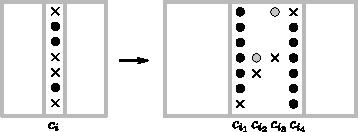
\includegraphics[width=0.6\textwidth]{split-ex.pdf} 
		\caption{Illustration of $S'$ in the proof of \Cref{lem:split is safe}. The symbols $\times$ denote accesses and circles are touched points.}
		\label{fig:split}
	\end{figure}

	
	It is easy to verify that, after placing these points, the set is
	still satisfied. The number of points placed in these columns is exactly
	$2p_{i}+2(m_{i}-2) $. Thus after applying this modification to every
	column $c_{i}$, there are at most $2\opt(X)+2m\le4\opt(X)$ points. 
\end{proof}
Now we are ready to prove the main theorem.


\begin{proofof}{ \Cref{thm:perm-all}}
	First, we have that $ \cA_{T}(X)  \le  \cA_{T}^{p,\mathit{ins}}( X^{p,\mathit{ins}}) $
	because $\merge$ never increases the number of points. 
	We conclude that
	\[
	\cA_{T}(X)  \le  \cA_{T}^{p,\mathit{ins}}( X^{p,\mathit{ins}} ) = \cA_{T^p}^p( X^p )  \leq c\opt(\Split(X)) \le4c\opt(X)
	,\]
	where the second inequality follows from \Cref{lem:bounded by access-only}, 
	the third inequality follows from the assumption that $\cA^p$ is $c$-competitive for only accessing on only permutations, 
	and the last inequality follows from \Cref{lem:split is safe}, and hence $\cA$ is a $4c$-competitive
	online BST for any access sequence.
	\end{proofof}
